\begin{frame}
    \frametitle{Présentation de l'API}
    \begin{center}
	      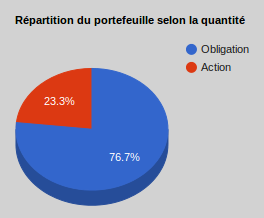
\includegraphics[scale=0.395]{images/google2.png}
	      \hskip1em
	      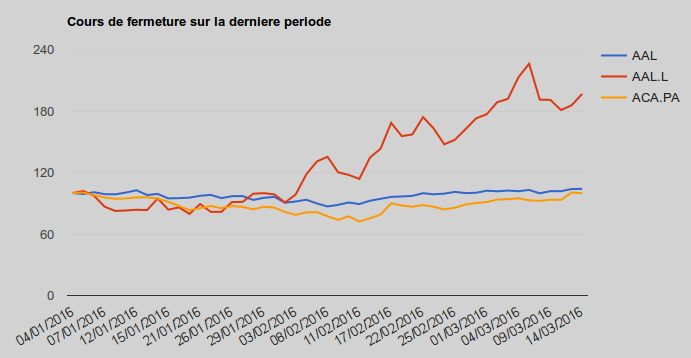
\includegraphics[scale=0.24]{images/google1.png}
    \end{center}
    \begin{block}{Avantages de l'API}
    	\begin{itemize}
    		\item Graphes intéractifs
    		\item Directement dans la JSP avec JavaScript
    	\end{itemize}
    \end{block}
\end{frame}

\begin{frame} [fragile]
    \frametitle{Présentation de l'API}
    \begin{enumerate}
     \item Charger la librairie :
\begin{lstlisting}[language=HTML, basicstyle=\scriptsize] 
<script type="text/javascript"
src="https://www.gstatic.com/charts/loader.js"></script>
<script type="text/javascript">
google.charts.load('current', {packages: ['corechart']});
google.charts.setOnLoadCallback(drawChart);
</script>
\end{lstlisting}	
     \item Préparer les données : créer une DataTable.
\begin{lstlisting}[language=HTML, basicstyle=\scriptsize] 
var data = new google.visualization.DataTable();
data.addColumn('string', 'Actifs');
data.addColumn('number', 'Quantite');
data.addRows([ ['Obligation', 76.7],['Action', 23.3]]);
\end{lstlisting}
 
    \end{enumerate}
\end{frame}

\begin{frame} [fragile]
    \frametitle{Présentation de l'API}
    \begin{enumerate}
     \setcounter{enumi}{2}
     \item Personnaliser le graphe : titre, dimensions, couleurs,...
\begin{lstlisting}[language=JAVA, basicstyle=\scriptsize]      
var options = { title: 'Repartition portefeuille'};
\end{lstlisting}    
     \item Dessiner le graphe : choix du type de graphe.
\begin{lstlisting}[language=JAVA, basicstyle=\scriptsize]      
var chart = new google.visualization.PieChart(
  document.getElementById('camembert'));
chart.draw(data, options);
\end{lstlisting}    
     \item Afficher le graphe : choisir l'emplacement dans la page HTML.
\begin{lstlisting}[language=HTML, basicstyle=\scriptsize]      
<div id="camembert"></div>
\end{lstlisting}    
    \end{enumerate}
\end{frame}